\documentclass[12pt,a4paper]{article}
\usepackage{physics}
\usepackage{amssymb}
\usepackage{subcaption}
\usepackage{colortbl}
\usepackage{musicography}
\newcommand{\activity}{Activity 10 -- Blob analysis}
\input{spp.dat}

\begin{document}

\title{\TitleFont \activity}
\author[ ]{\textbf{Kenneth V. Domingo} \\
2015--03116 \\
App Physics 186, 1\textsuperscript{st} Semester, A.Y. 2019--20}
\affil[ ]{\corremail{kvdomingo@up.edu.ph} }

\maketitle
\thispagestyle{titlestyle}

\section*{Results and Discussion}
\setcounter{section}{1}
For this activity \cite{soriano}, we'll use the provided image of a cell. First, we convert it to grayscale (Fig. \ref{fig:cell-gray}) and obtain its histogram (Fig. \ref{fig:gray-hist}). Notice that there is a huge peak somewhere between the 200 and 250 grayscale values, and another relatively smaller peak at around 200. We can interpret the huge peak as the background values and the small peak as the cell values. Thus, we can use Otsu's method to automatically select the best threshold value. From here, we can use the \texttt{skimage} library to automatically detect the blobs and label them. Each detected unique blob is labeled by assigning it a unique integer. A total of 150 blobs were detected. The result of the blob detection and labeling is shown in Fig. \ref{fig:cell-blobs}, and its grayscale histogram in Fig. \ref{fig:blobs-hist}. Note that Otsu's method was able to separate the two peaks.

Initial inspection of the blob detection showed that there were some smaller blobs being detected. Using the \texttt{regionprops} function to obtain the blob areas, it was observed that there was a fairly narrow peak at around 175 px$^2$, with some outlier values $< 100$ and $> 300$ px$^2$. We then perform filtering by blob area such that only blobs with $100 < A < 300$ px$^2$ remain. The final area histogram is shown in Fig. \ref{fig:blob-area}. This distribution gives us a best estimate of the cell area of $\boxed{A = 172 \pm 26$ px$^2}$.

We also obtain the eccentricities of the blobs and filter them this time by the best estimate of the blob area. The resulting histogram is shown in Fig. \ref{fig:blob-ecc}. The best estimate for the eccentricity of the filtered blobs is $\boxed{e = 0.47 \pm 0.25}$. This means that most of the blobs, even those that appear circular in Fig. \ref{fig:cell-blobs}, are ever so slightly elliptical.

We also obtain the major axis lengths---which we will essentially treat as the blob diameter---of the the blobs and filter them again by the best estimate of the blob area. The resulting histogram is shown in Fig. \ref{fig:blob-majax}. The best estimate for the major axis lengths of the filtered blobs is $\boxed{2a = 16 \pm 1$ px$}$. This shows that the cell blobs do not vary much in diameter.

Finally, we obtain the perimeter of the blobs. Following the same procedures as before, we obtain a histogram in Fig. \ref{fig:blob-per} and a best estimate of the perimeter $\boxed{P = 59 \pm 10$ px$}$.

\begin{figure}[htb]
	\centering
	\begin{subfigure}[h!]{0.49\textwidth}
		\centering
		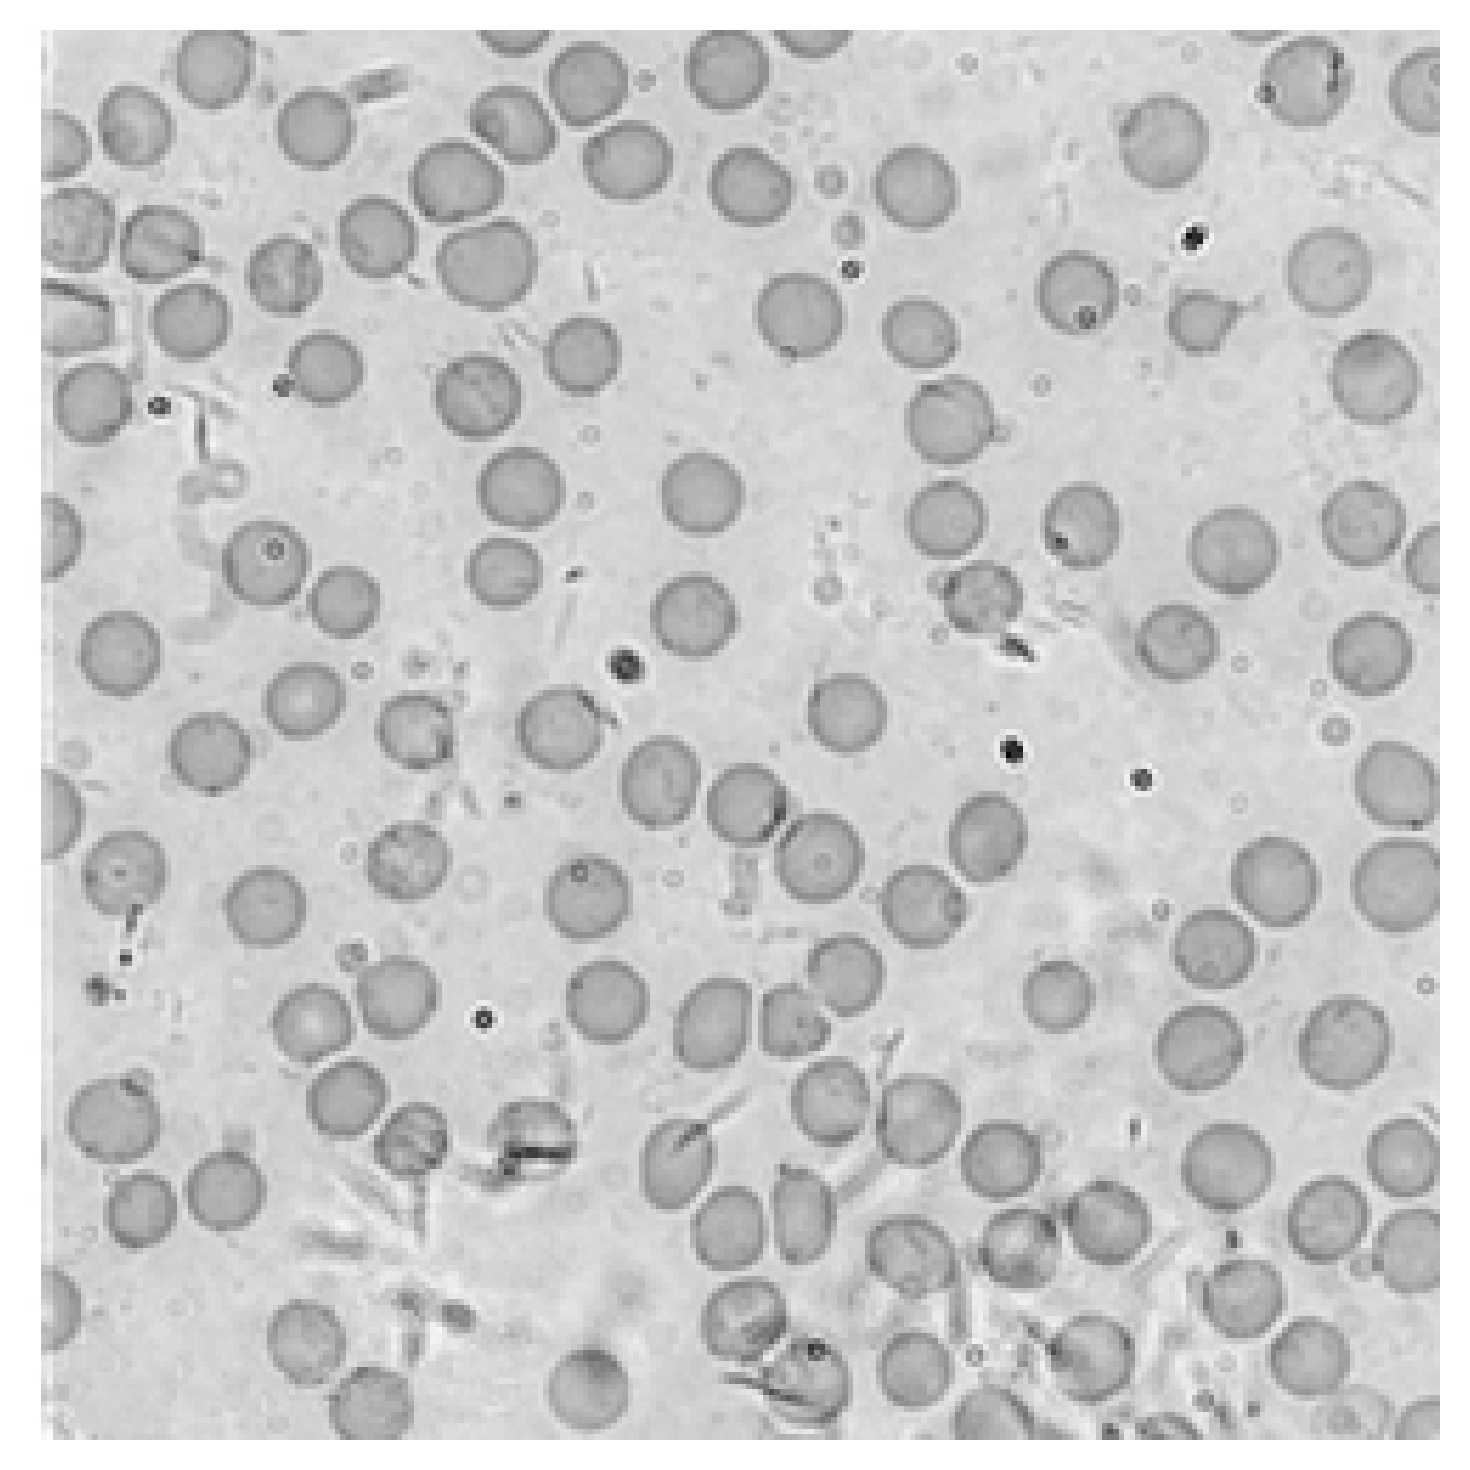
\includegraphics[width=\textwidth]{cell_gray.png}
		\caption{}
		\label{fig:cell-gray}
	\end{subfigure}
	\begin{subfigure}[h!]{0.49\textwidth}
		\centering
		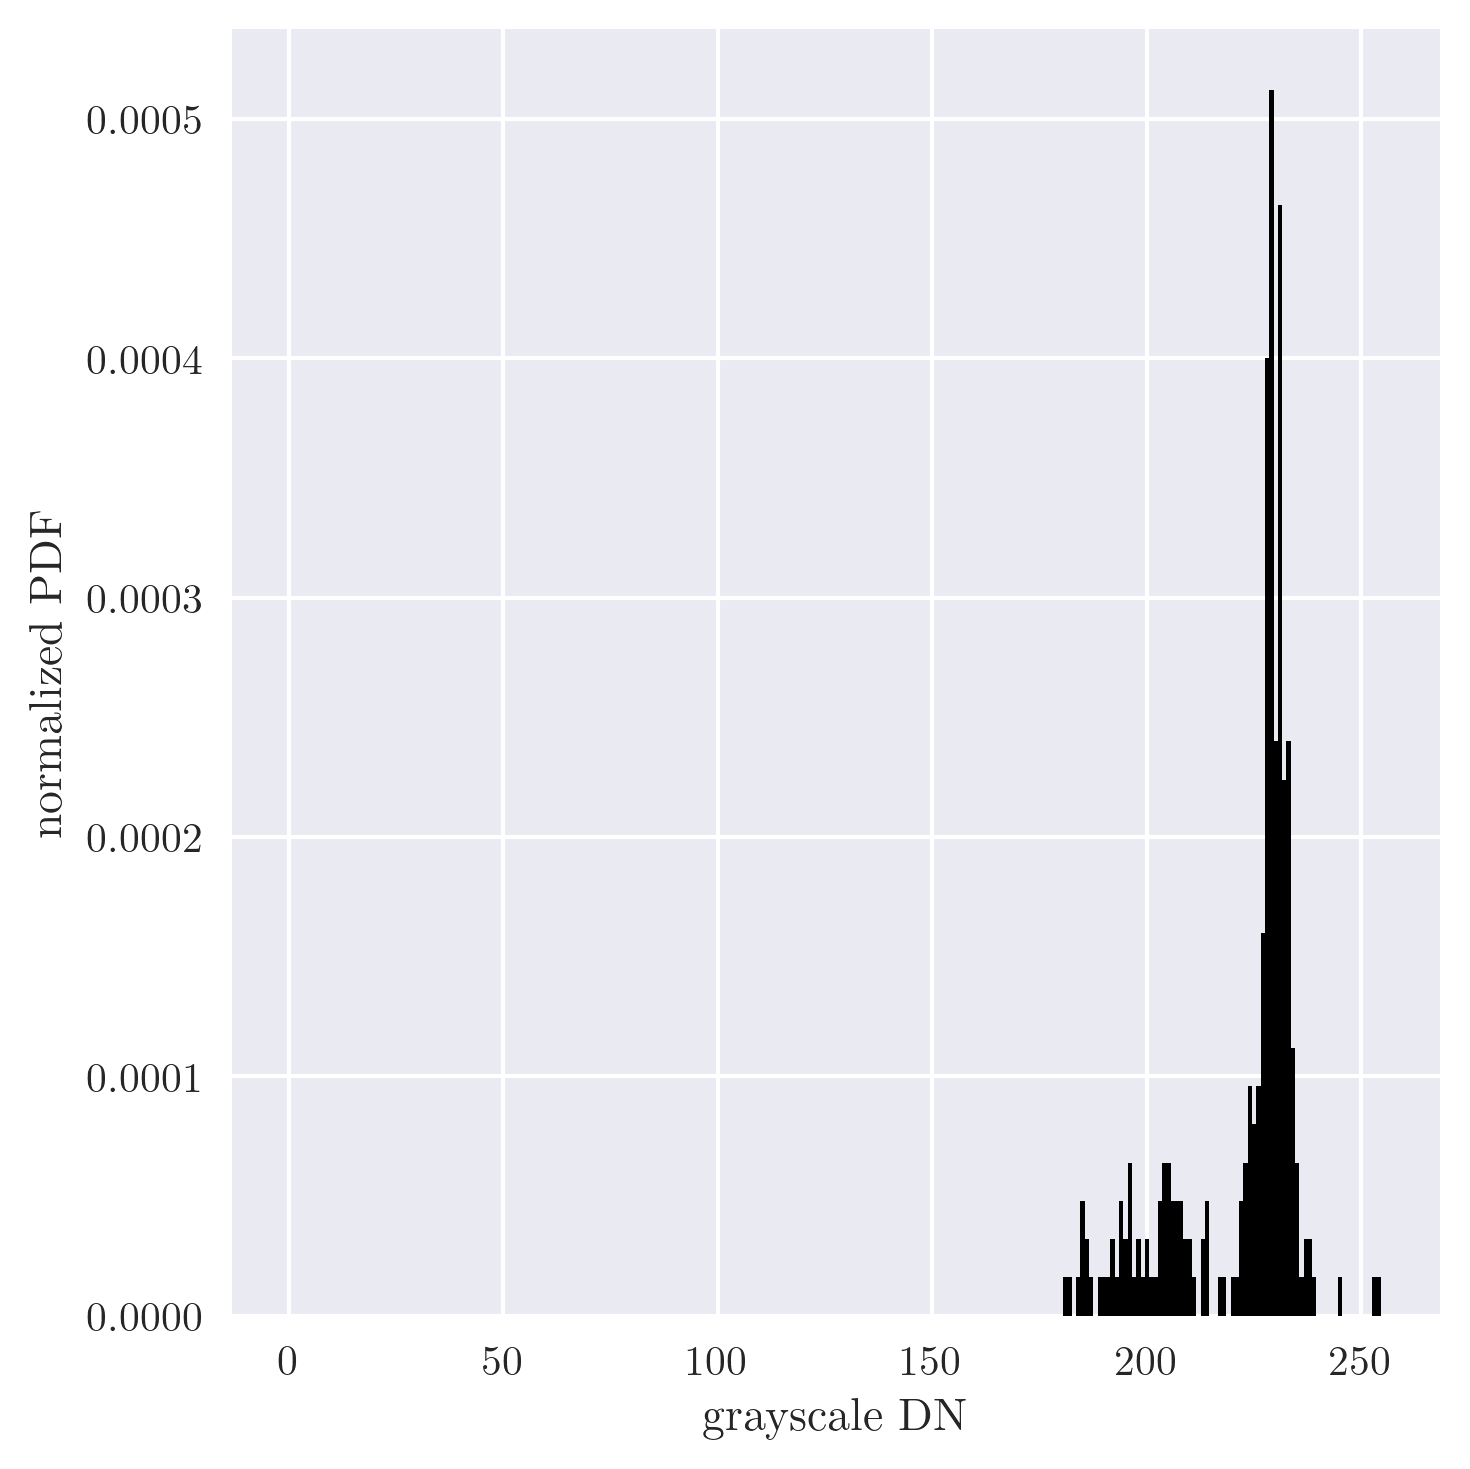
\includegraphics[width=\textwidth]{gray_hist.png}
		\caption{}
		\label{fig:gray-hist}
	\end{subfigure}
	\begin{subfigure}[h!]{0.49\textwidth}
		\centering
		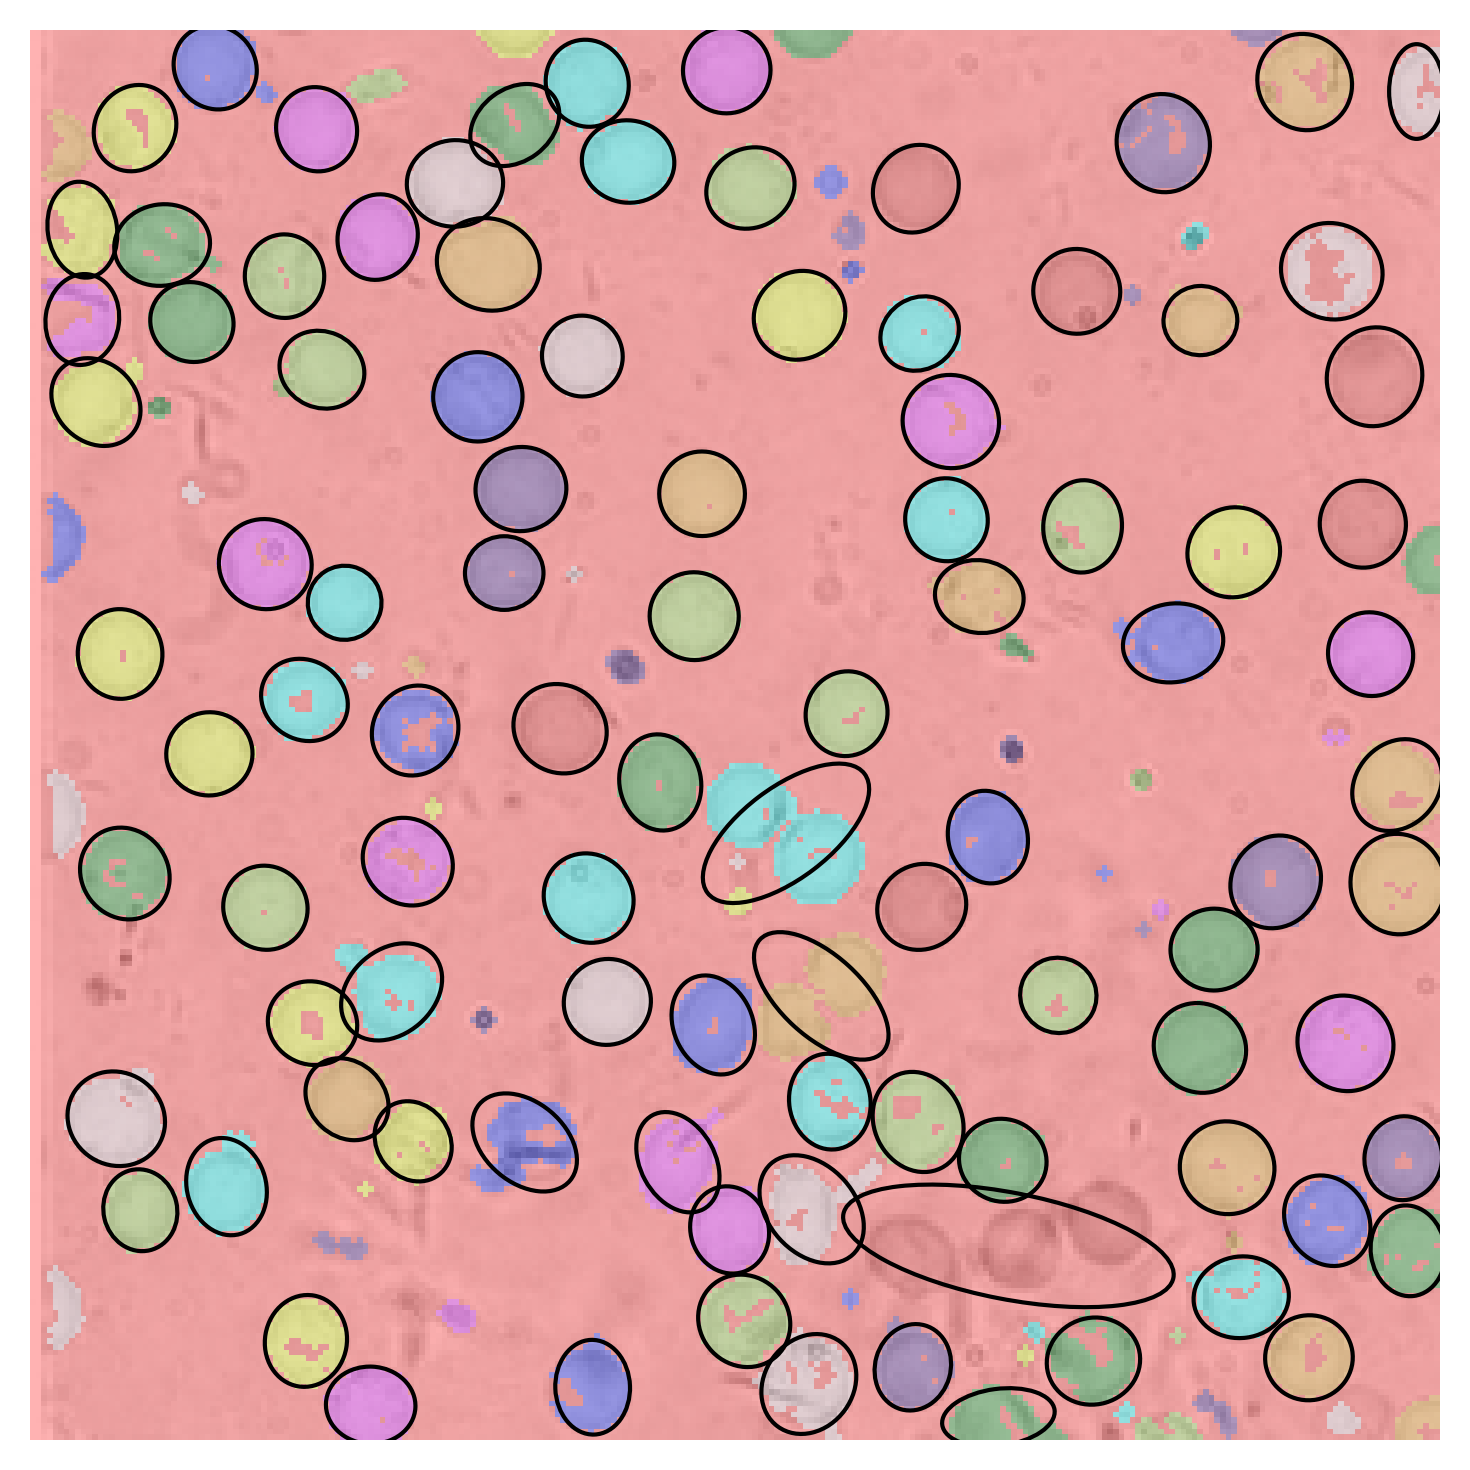
\includegraphics[width=\textwidth]{cell_blobs.png}
		\caption{}
		\label{fig:cell-blobs}
	\end{subfigure}
	\begin{subfigure}[h!]{0.49\textwidth}
		\centering
		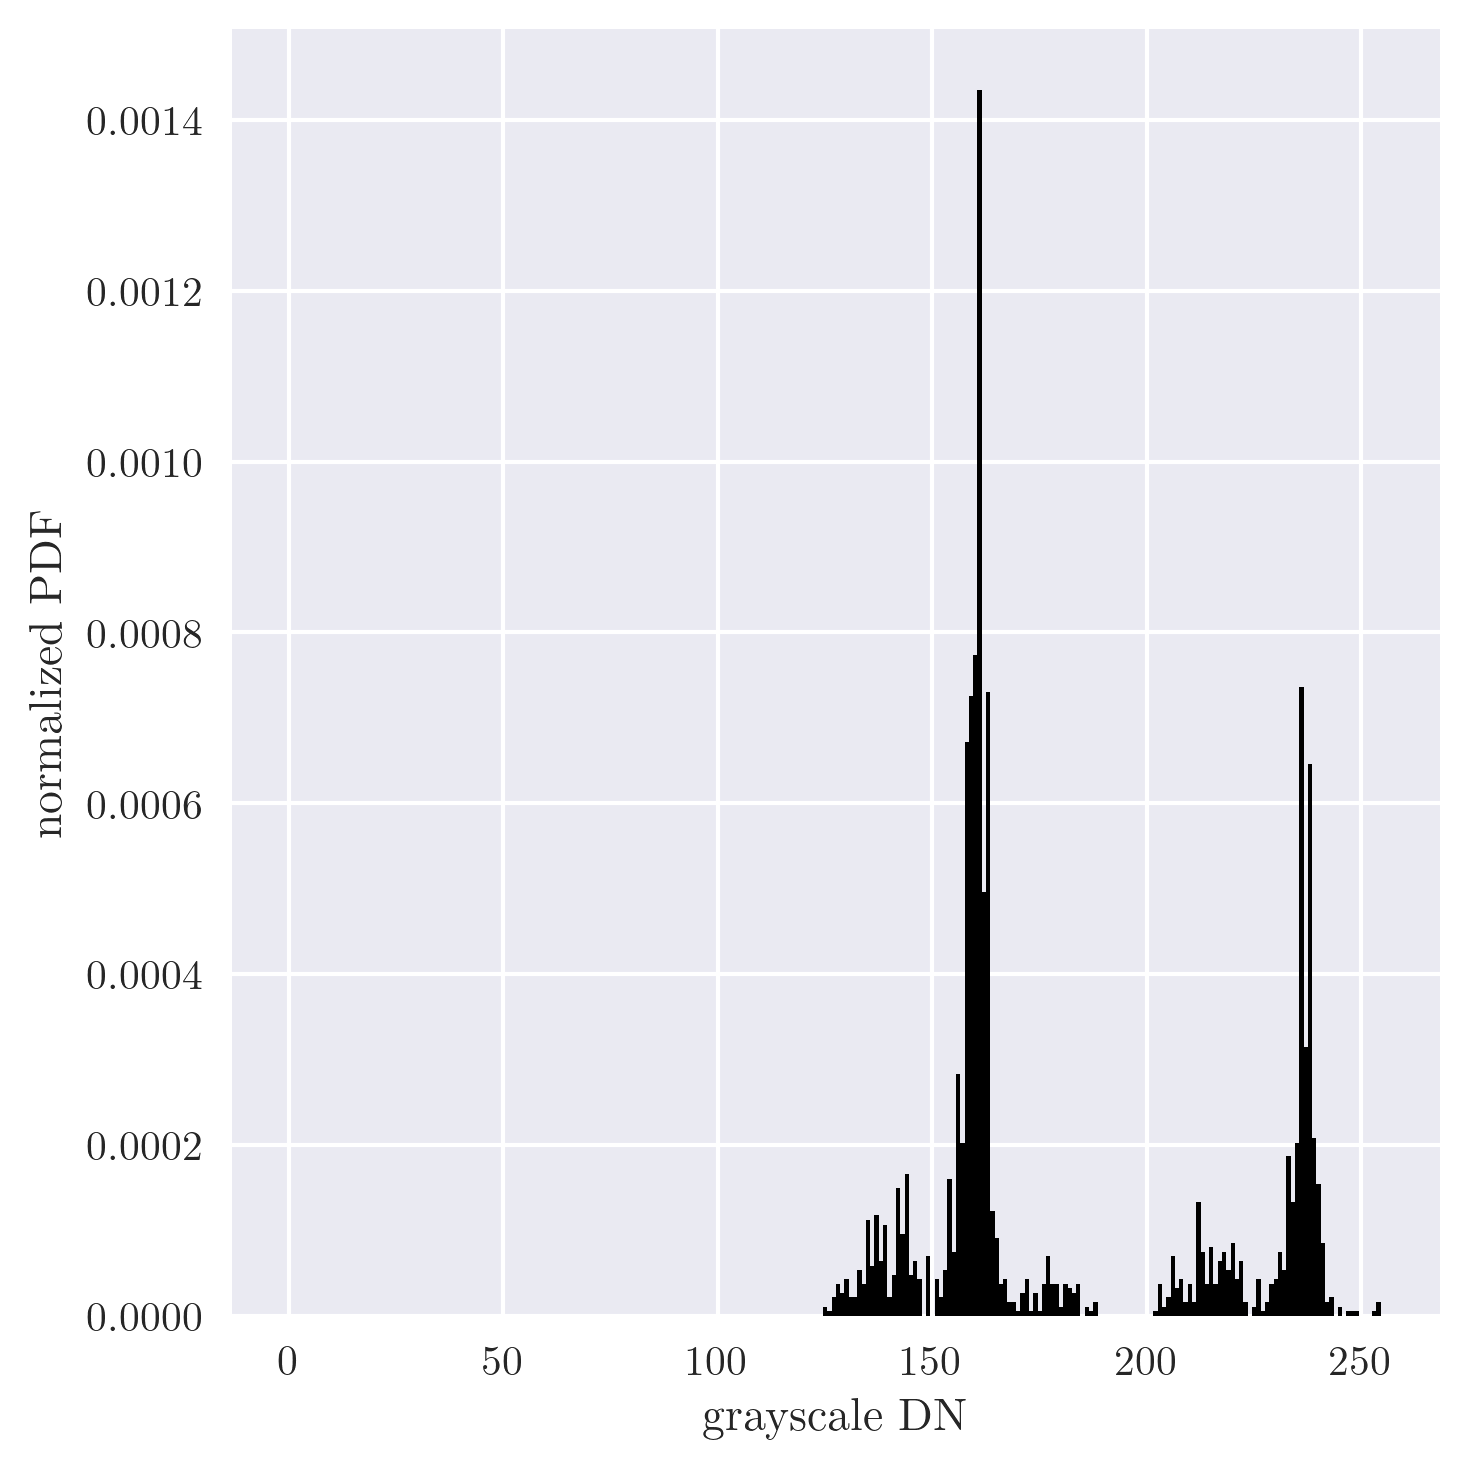
\includegraphics[width=\textwidth]{blobs_hist.png}
		\caption{}
		\label{fig:blobs-hist}
	\end{subfigure}
	\caption{(a) Grayscaled cell image, (b) grayscale histogram, (c) Filtered and labeled cell blobs, and (d) cell blobs histogram.}
	\label{fig:cell}
\end{figure}

\begin{figure}[htb]
	\centering
	\begin{subfigure}[h!]{0.49\textwidth}
		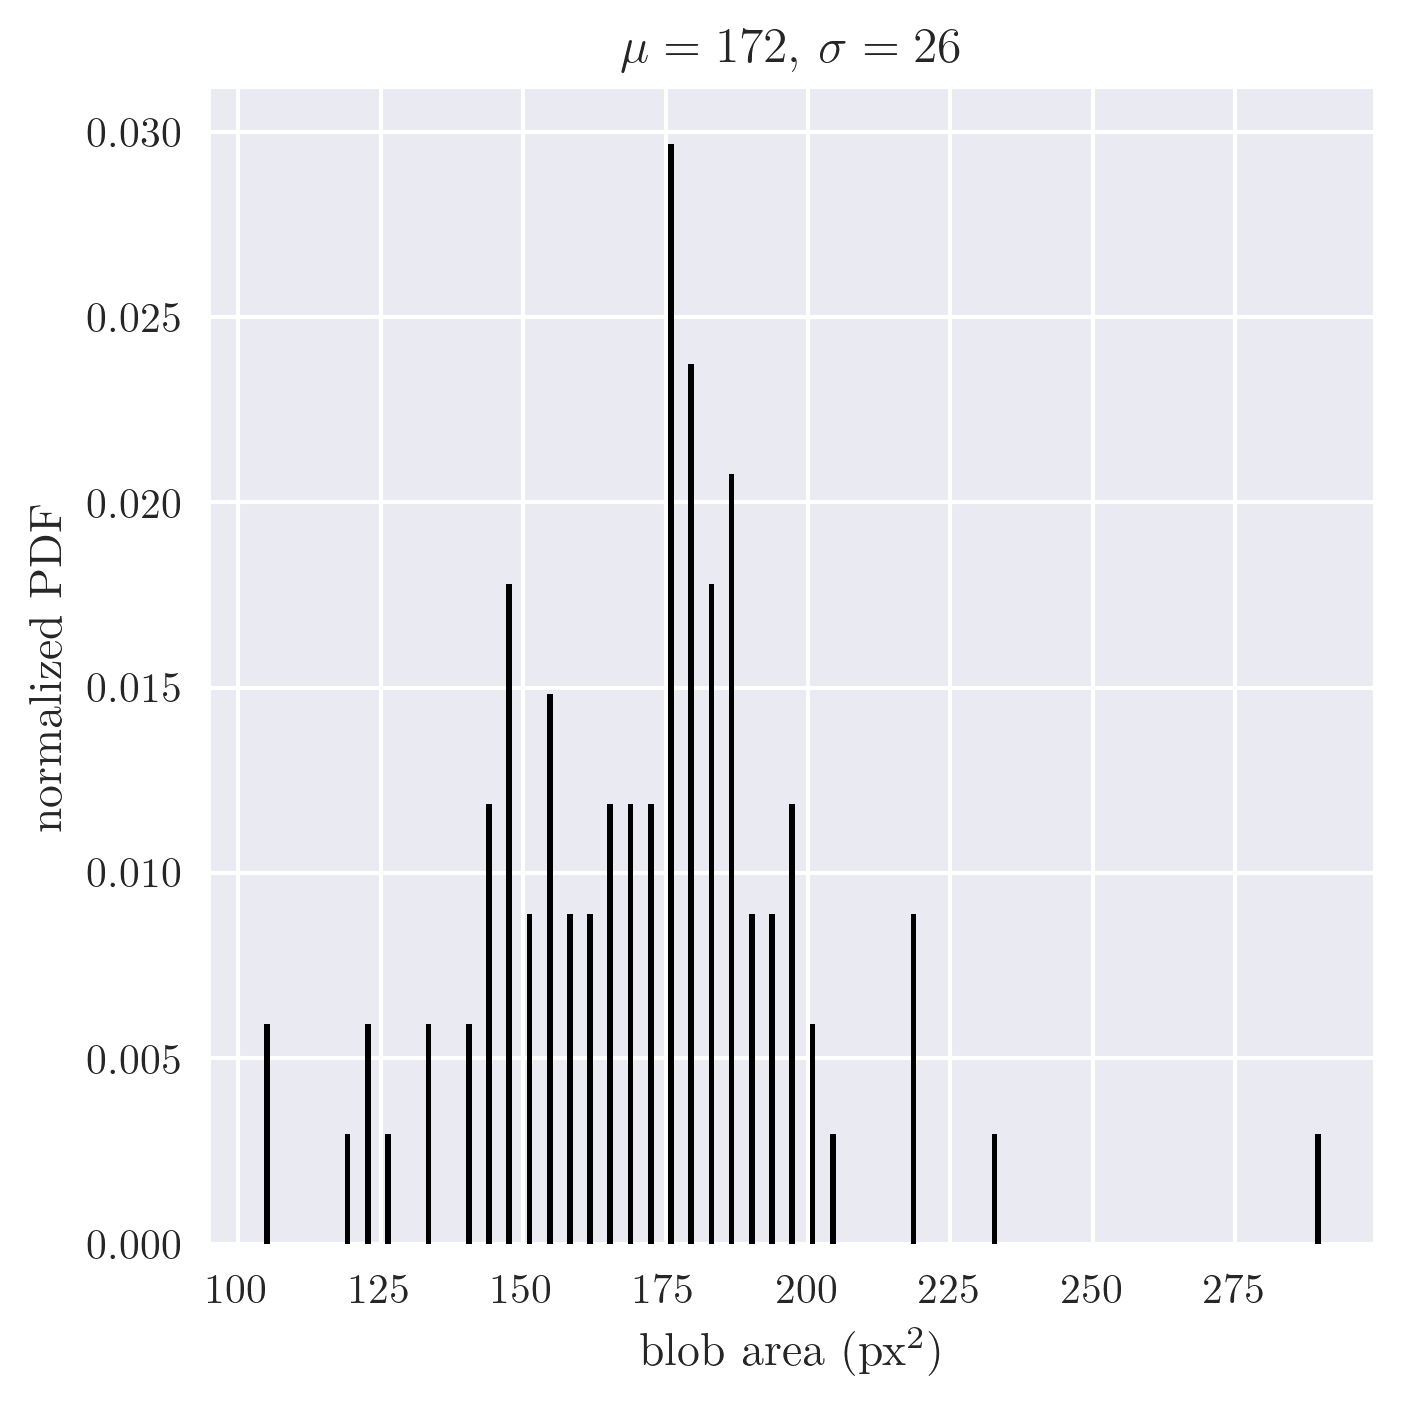
\includegraphics[width=\textwidth]{area_hist.png}
		\caption{area}
		\label{fig:blob-area}
	\end{subfigure}
	\begin{subfigure}[h!]{0.49\textwidth}
		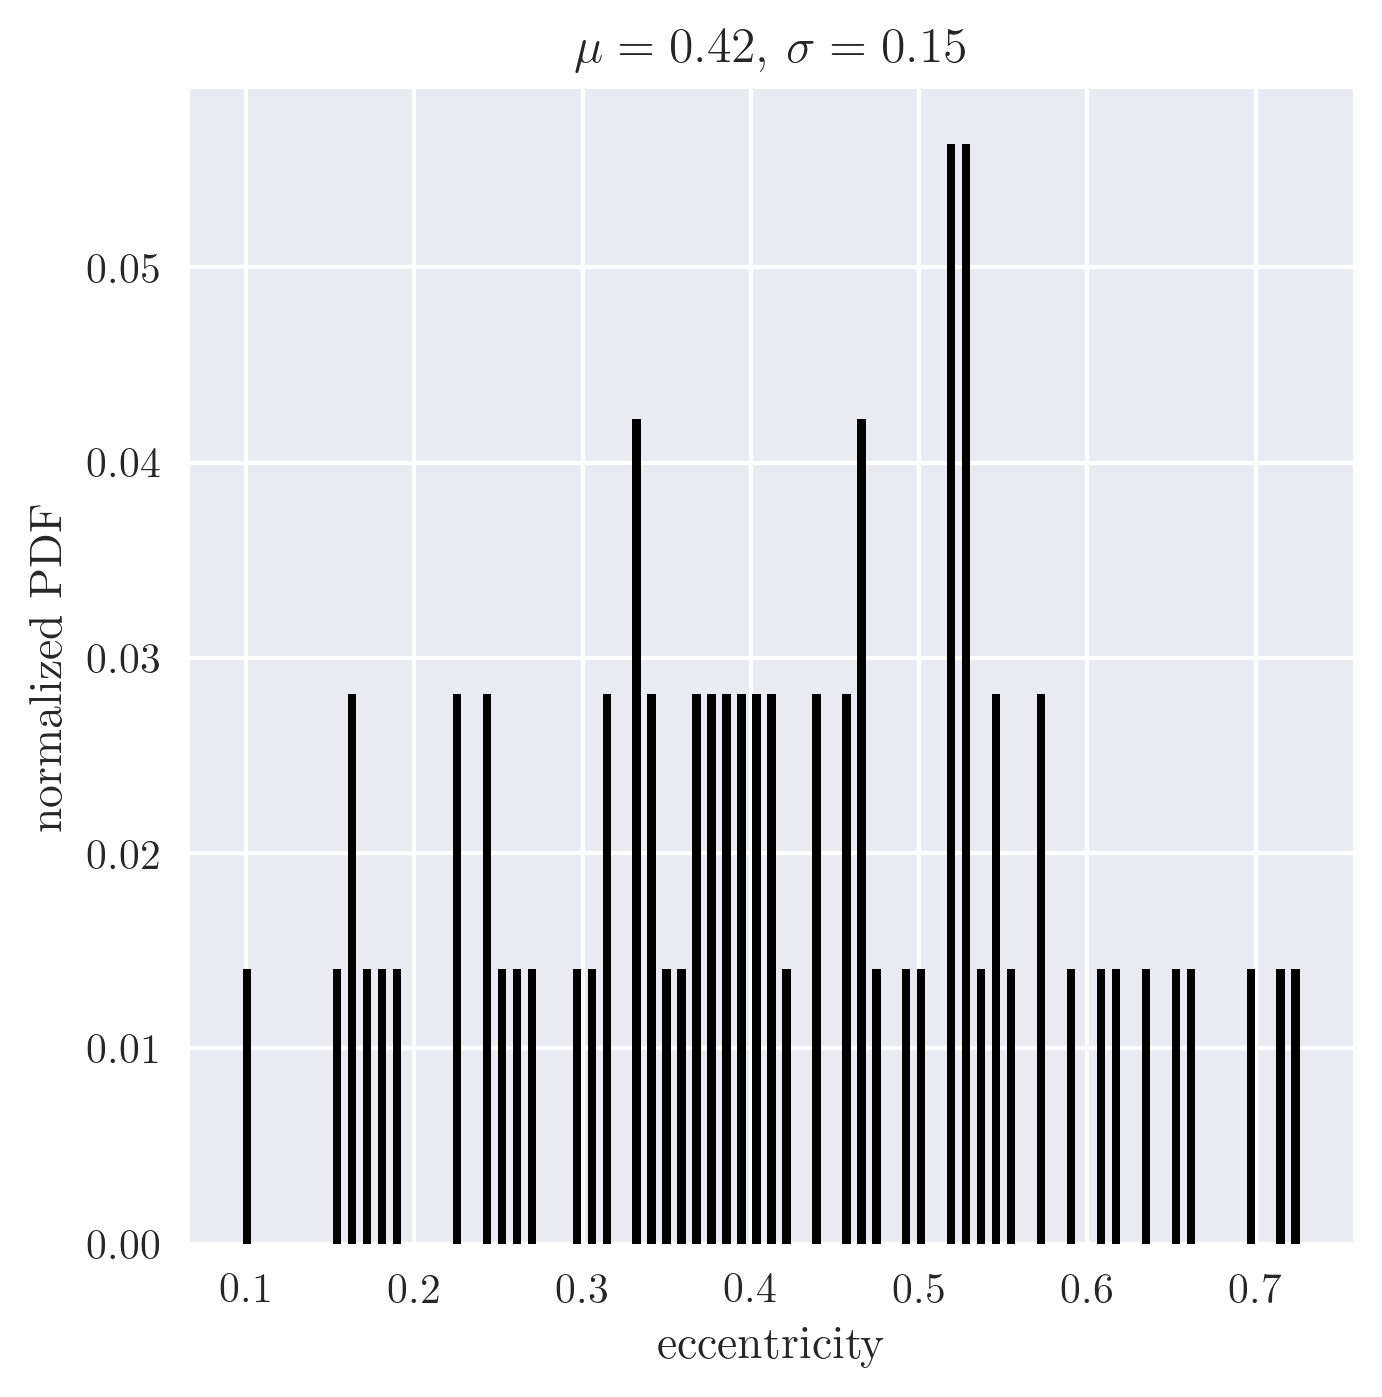
\includegraphics[width=\textwidth]{ecc_hist.png}
		\caption{eccentricity}
		\label{fig:blob-ecc}
	\end{subfigure}
	\begin{subfigure}[h!]{0.49\textwidth}
		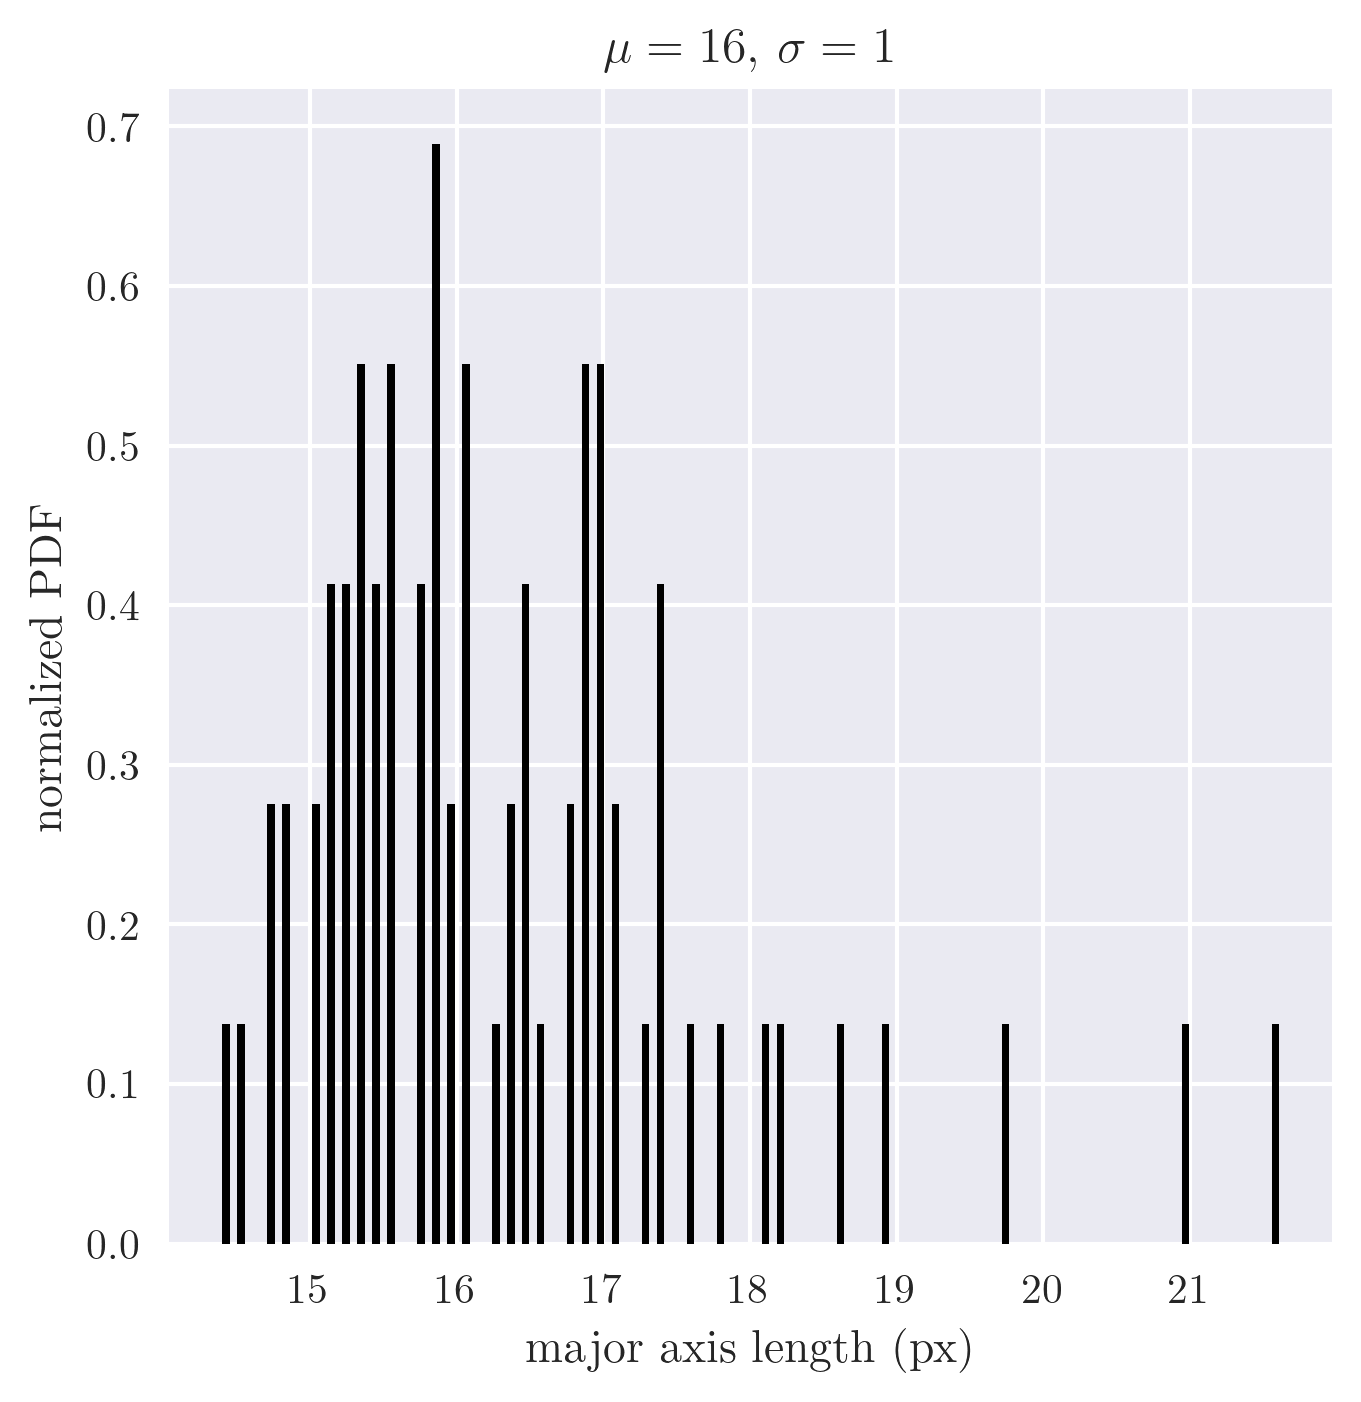
\includegraphics[width=\textwidth]{majax_hist.png}
		\caption{major axis length}
		\label{fig:blob-majax}
	\end{subfigure}
	\begin{subfigure}[h!]{0.49\textwidth}
		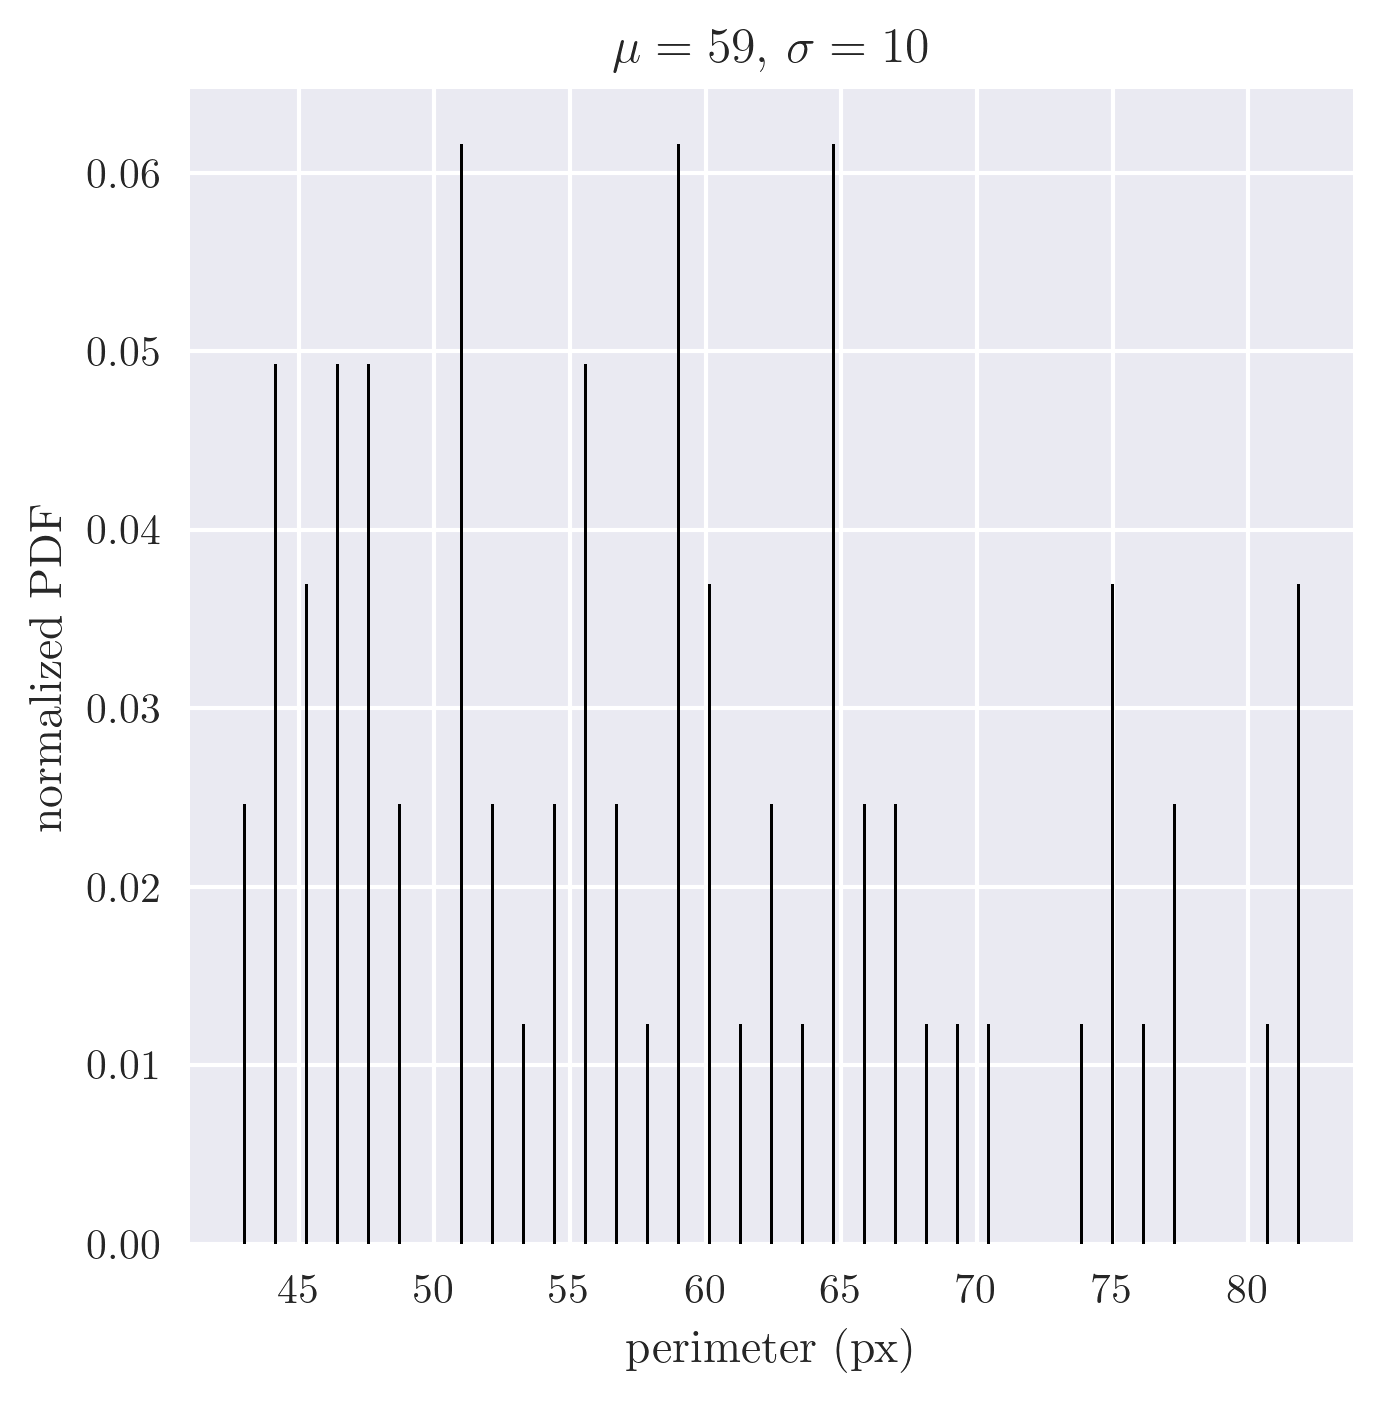
\includegraphics[width=\textwidth]{per_hist.png}
		\caption{perimeter}
		\label{fig:blob-per}
	\end{subfigure}
	\caption{Histogram of the blob properties.}
	\label{fig:blob-props}
\end{figure}


\clearpage
\begin{table}[!htb]
	\centering
	\caption{Self-evaluation.}
	\begin{tabular}{||r|c||}
		\hline
		Technical correctness & 5 \\ \hline
		Quality of presentation & 5 \\ \hline
		Initiative & 0 \\ \hline
		\textbf{TOTAL} & \textbf{10} \\ \hline
	\end{tabular}
	\label{tab:self-eval}
\end{table}

\bibliographystyle{spp-bst}
\bibliography{biblio}

\end{document}